In this section we evaluate the performance of our work-stealing framework built upon SALSA pools. 
We describe the experiment setup in Section~\ref{sec:exp-setup}, we show the overall system performance in Section~\ref{sec:eval-performance} and study the influence of SALSA techniques in Section~\ref{sec:eval-techniques}.

\subsection {Experiment Setup}
\label{sec:exp-setup}
We compare the following task pool implementations: 
\begin {itemize}
\item
{\bf WS-SALSA} -- our work-stealing framework with SCPool implemented by SALSA.
\item
{\bf WS-SALSAwCAS} -- our work-stealing framework with SCPool implemented by a simplistic SALSA variation, in which every {\bf consume()} and {\bf steal()} operation tries to take a single task using CAS. This way, SALSAwCAS isolates the effects of the low-synchronization fast-path and per-chunk stealing that are presented in SALSA.  
\item
{\bf ConcBag} -- our implementation of the lock-free concurrent bags algorithm~\cite{Sundell:2011:LAC:1989493.1989550}. 
No thread in our system acts as both a producer and a consumer, therefore every consume operation of a concurrent bags algorithm steals a task from some producer.
\item
{\bf WS-MSQ} -- our work-stealing framework with SCPool implemented by Michael-Scott non-blocking queue~\cite{Michael:1996:SFP:248052.248106} -- both {\bf consume()} and {\bf steal()} operations invoke the {\bf dequeue()} function of the queue. 
\item
{\bf WS-LIFO} -- our work-stealing framework with SCPool implemented by LIFO stack by Michael~\cite{Michael:2004:HPS:987524.987595}. 
%\item
%{\bf WSQ} -- Work stealing queues, which do not ensure FIFO. There is one CLQ per consumer. A producer chooses a random queue to insert a task; a consumer tries first to retrieve a task from its own queue, and if it fails, attempts to retrieve a task from the CLQ of another consumer. In the worst case, all consumer queues are checked.
\end {itemize} 

All the pools are implemented in C++ and compiled with \texttt{-O2} optimization level. 
In order to minimize the scalability issues related to the excessive memory allocations by WS-MSQ and WS-LIFO, we use \texttt{jemalloc} allocator~\cite{citeulike:4951109}, which was shown to be highly scalable in multi-threaded environments\footnote{\url{http://www.facebook.com/notes/facebook-engineering/scalable-memory-allocation-using-jemalloc/480222803919}}.
Unless stated otherwise, the chunk pools of SALSA and SALSAwCAS contain $1000$ tasks, the chunk pools of ConcBag contain $128$ tasks (the optimal values for these algorithms). 

We use a synthetic benchmark for performance evaluation, where 1) each producer works in a loop of inserting a dummy item; 2) each consumer works in a loop of retrieving dummy items. The results are the average of $5$ runs with duration of $20$ seconds. 
The tests are run on a dedicated shared memory NUMA server with $8$ Quad Core AMD $2.3$GHz processors and $16$GB of memory attached to each processor. 

\subsection{System Throughput}
\label{sec:eval-performance}

\begin{figure}[htb]
	\centering
	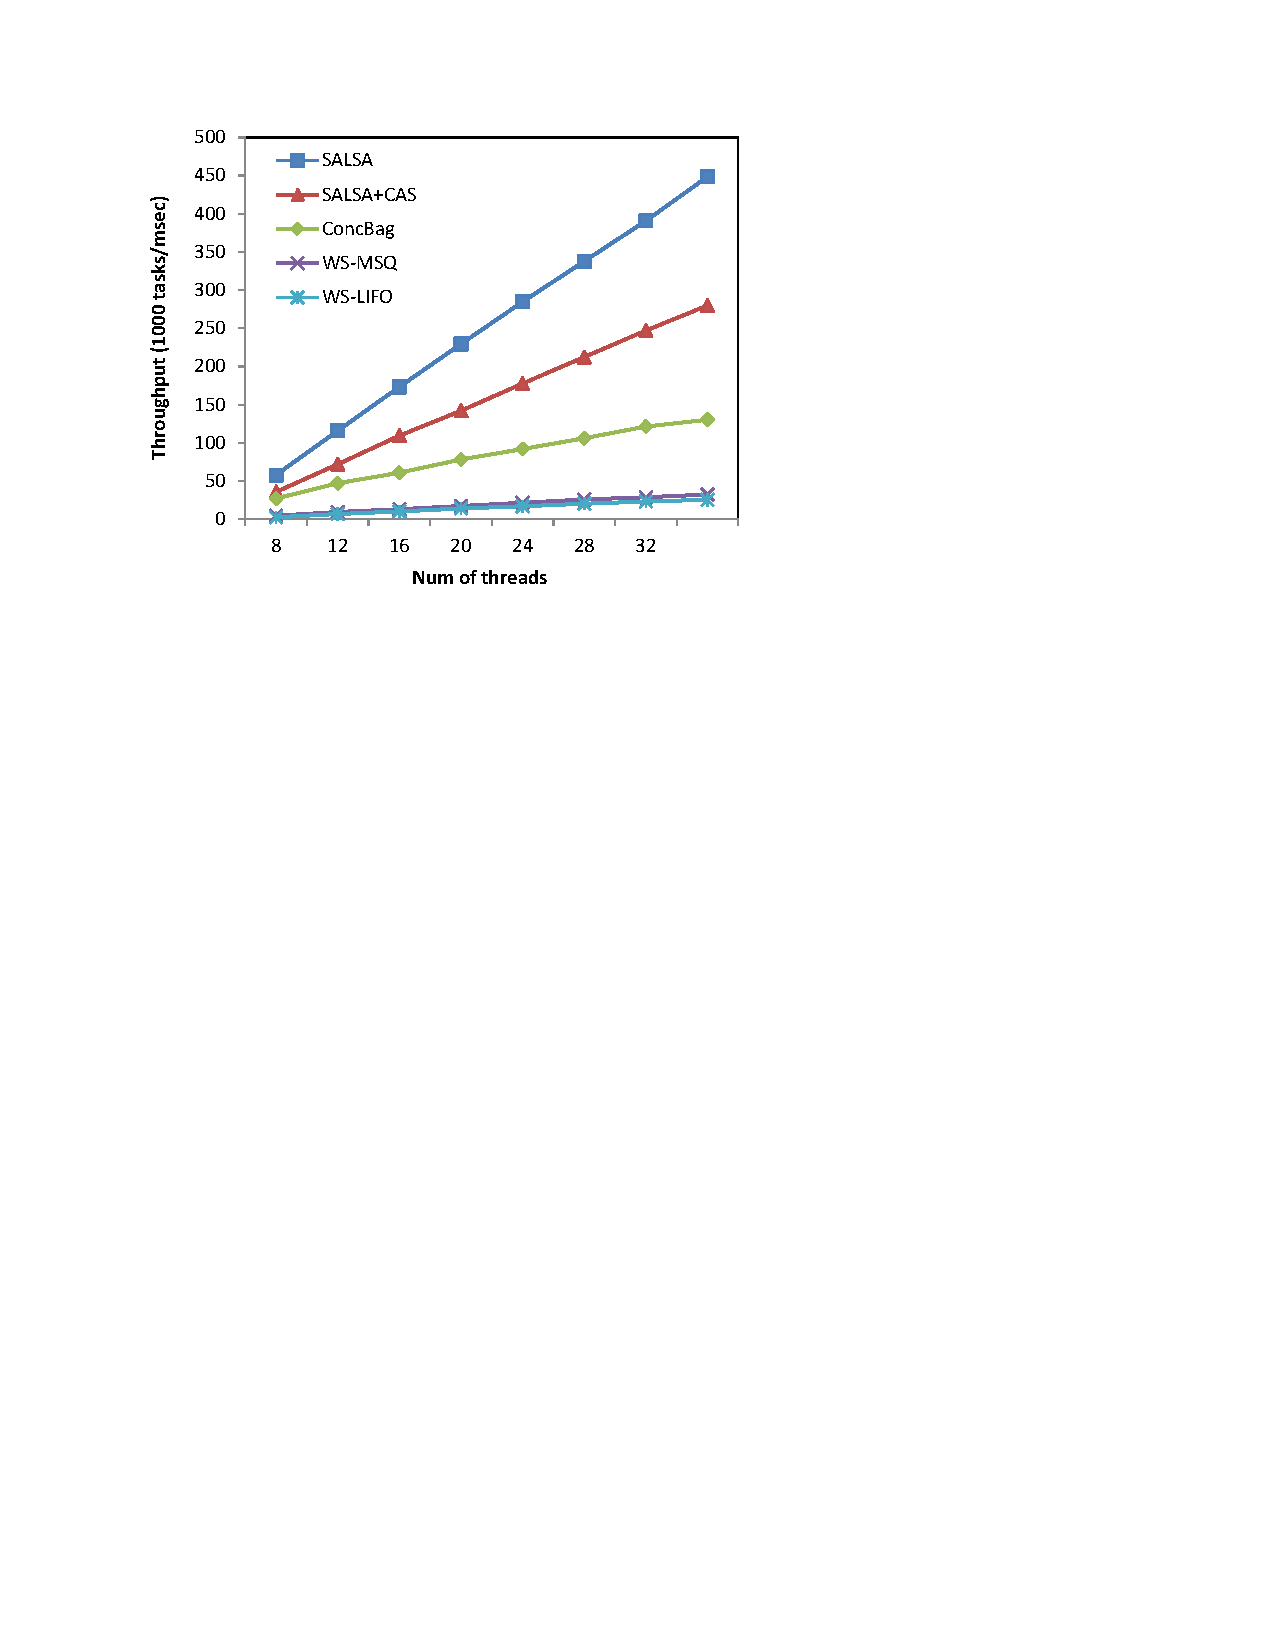
\includegraphics[width=0.40\textwidth]{figures/n-n-throughput}
  \caption{\footnotesize{System throughput for N/N workload. }}
	\label{fig:n-n-throughput}
\end{figure}

\begin{figure}[htb]
	\centering
  \subfigure [\scriptsize{System throughput (1/N workload).}] {
    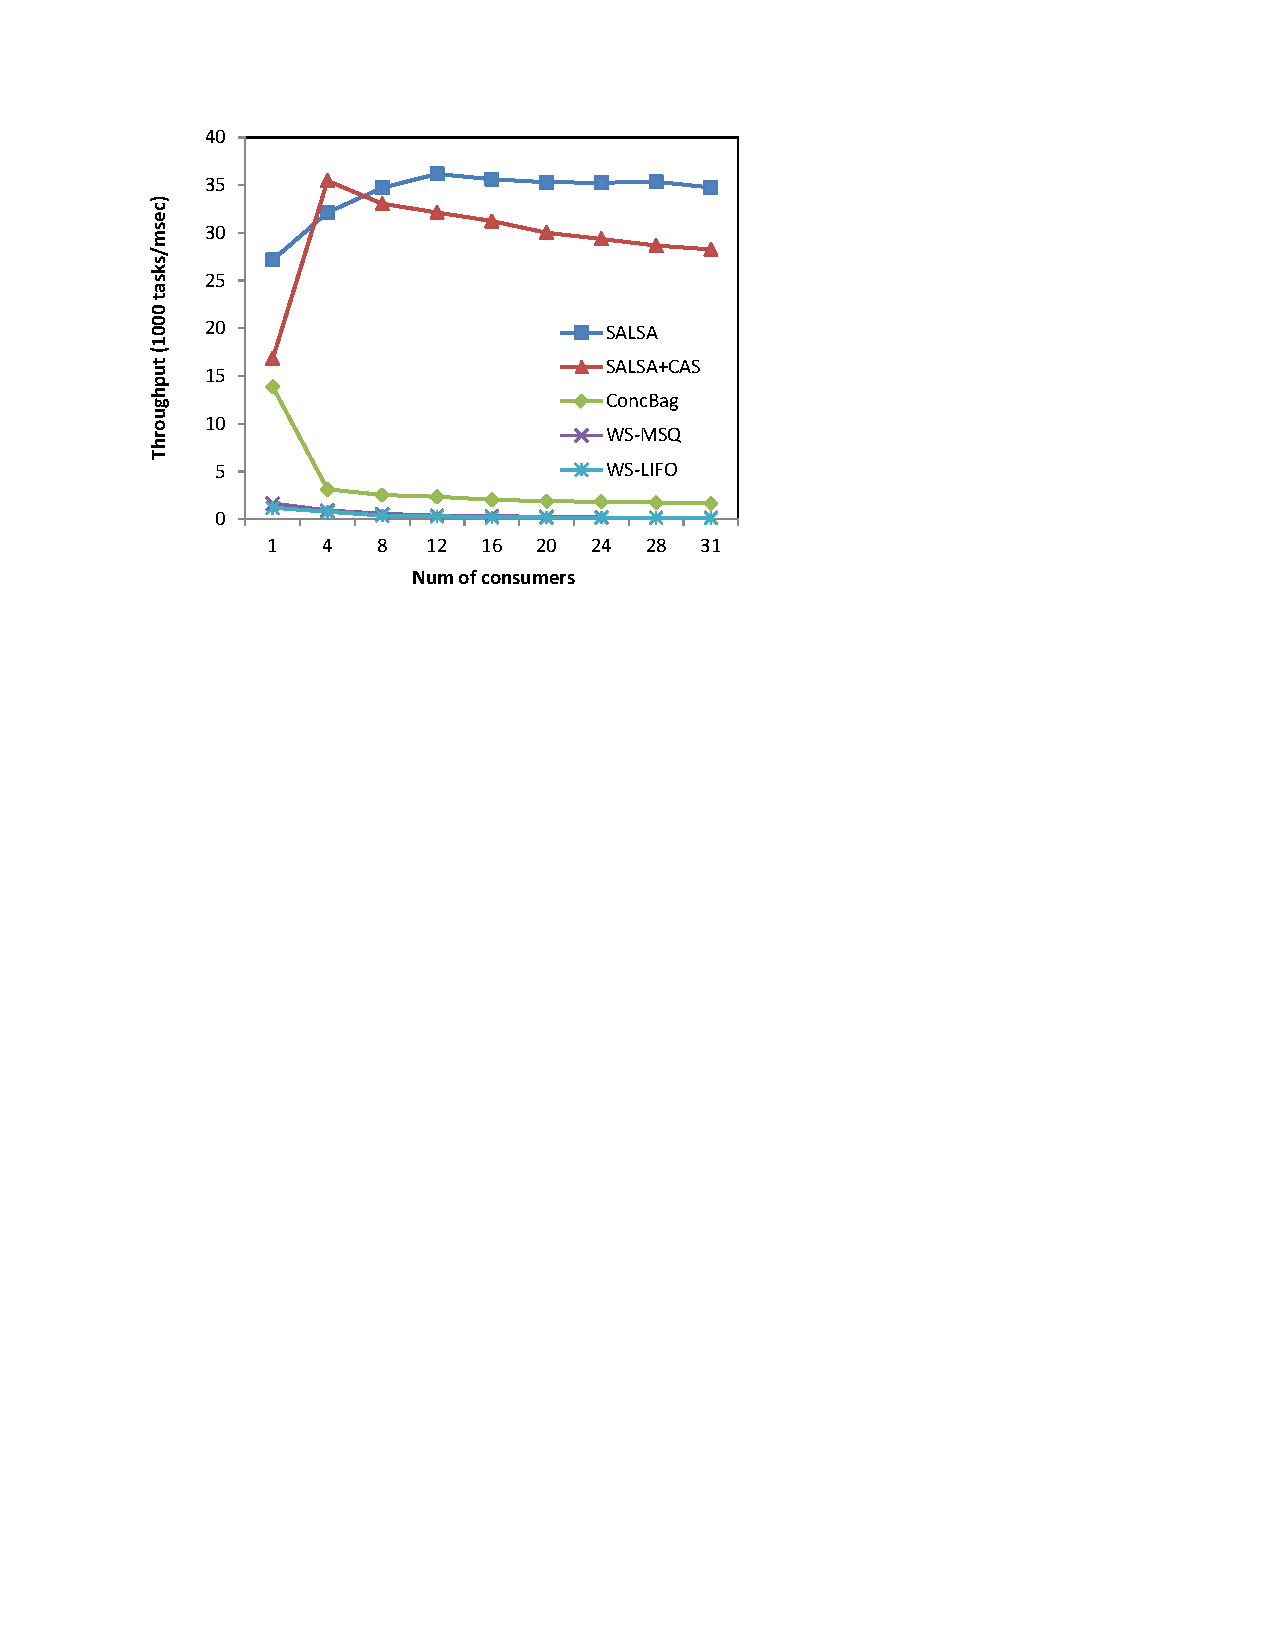
\includegraphics[width=0.40\textwidth]{figures/1-n-throughput}
    \label{fig:1-n-throughput}
  }
  \subfigure [\scriptsize{CAS operations per task retrieval (1/N workload).}] {
    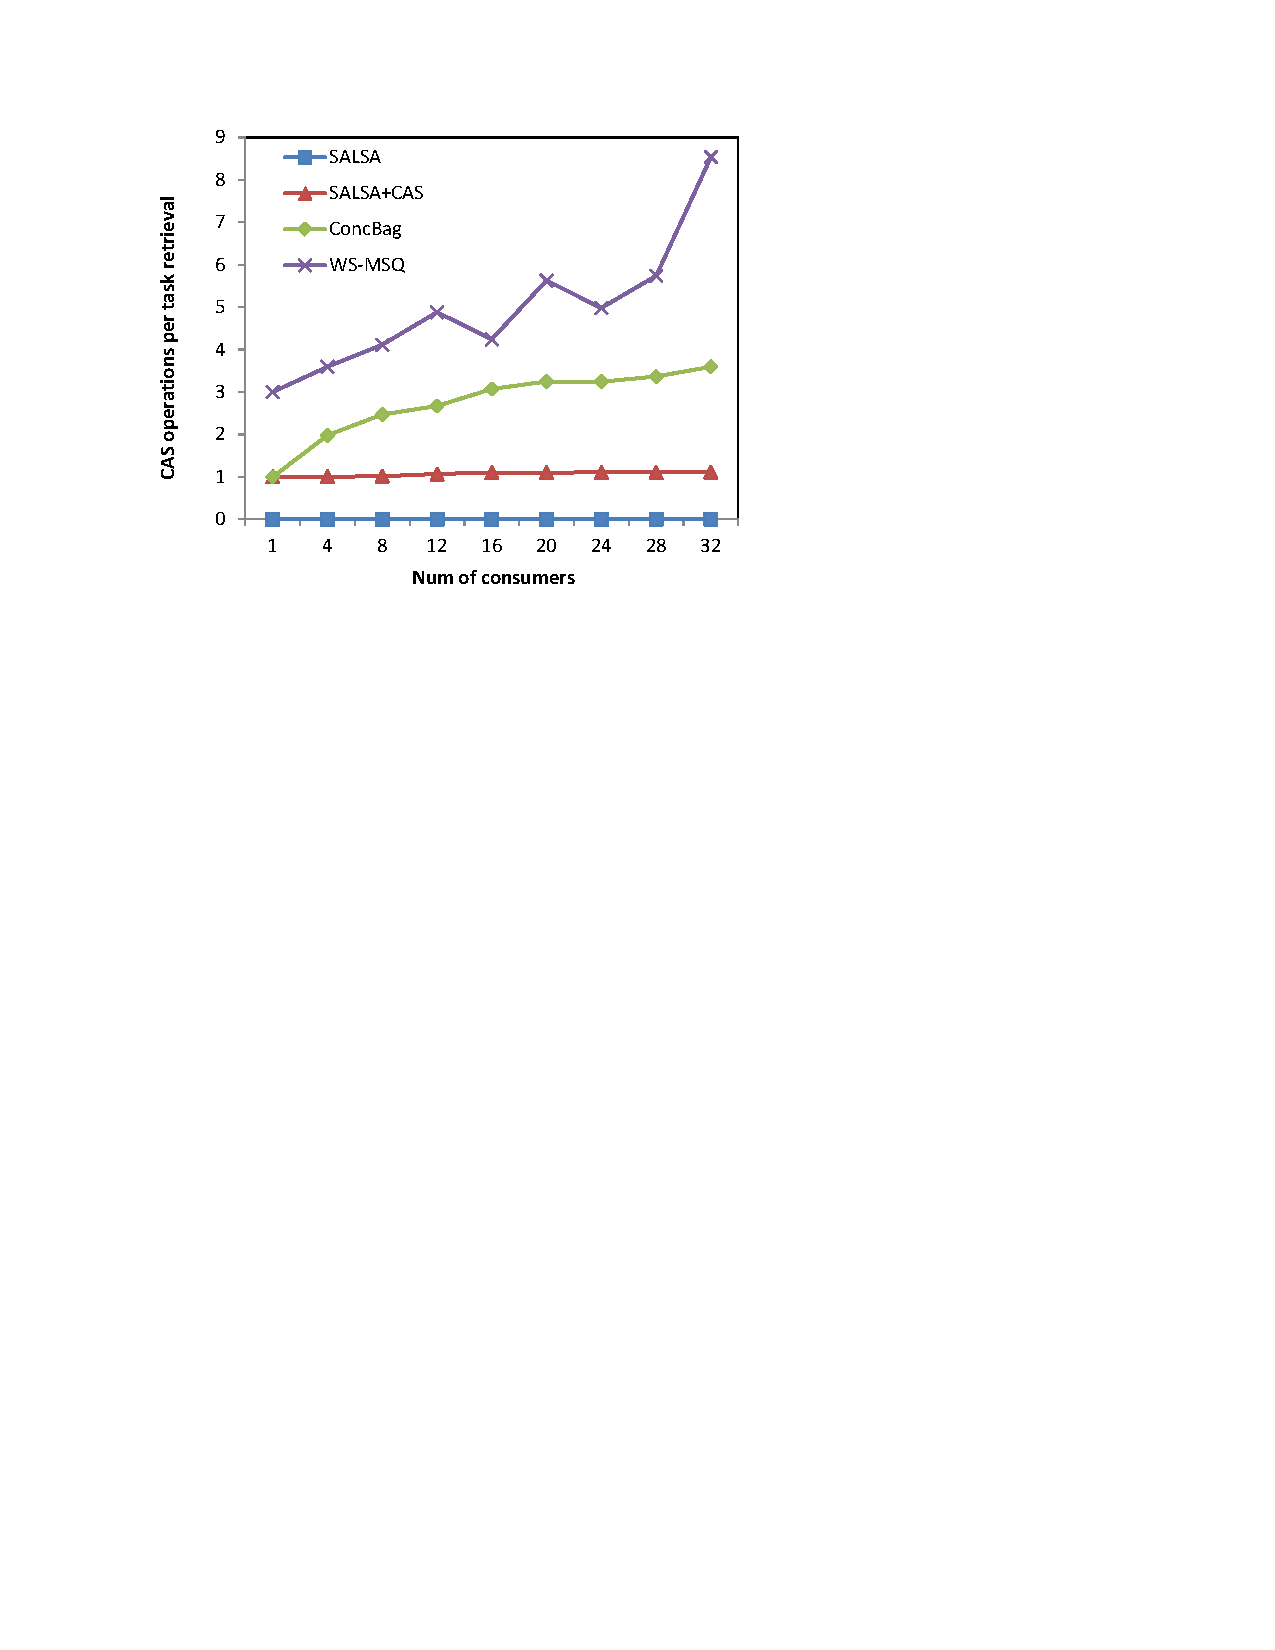
\includegraphics[width=0.40\textwidth]{figures/1-n-cas}
    \label{fig:1-n-cas}
  }
	\caption{\footnotesize{Single producer -- multiple consumers behavior. }}
	\label{fig:1-n-perf}
\end{figure}

\subsection{SALSA Parameters Study}
\label{sec:eval-techniques}

\begin{figure}[htb]
	\centering
  \subfigure [\scriptsize{System throughput (1/N workload).}] {
    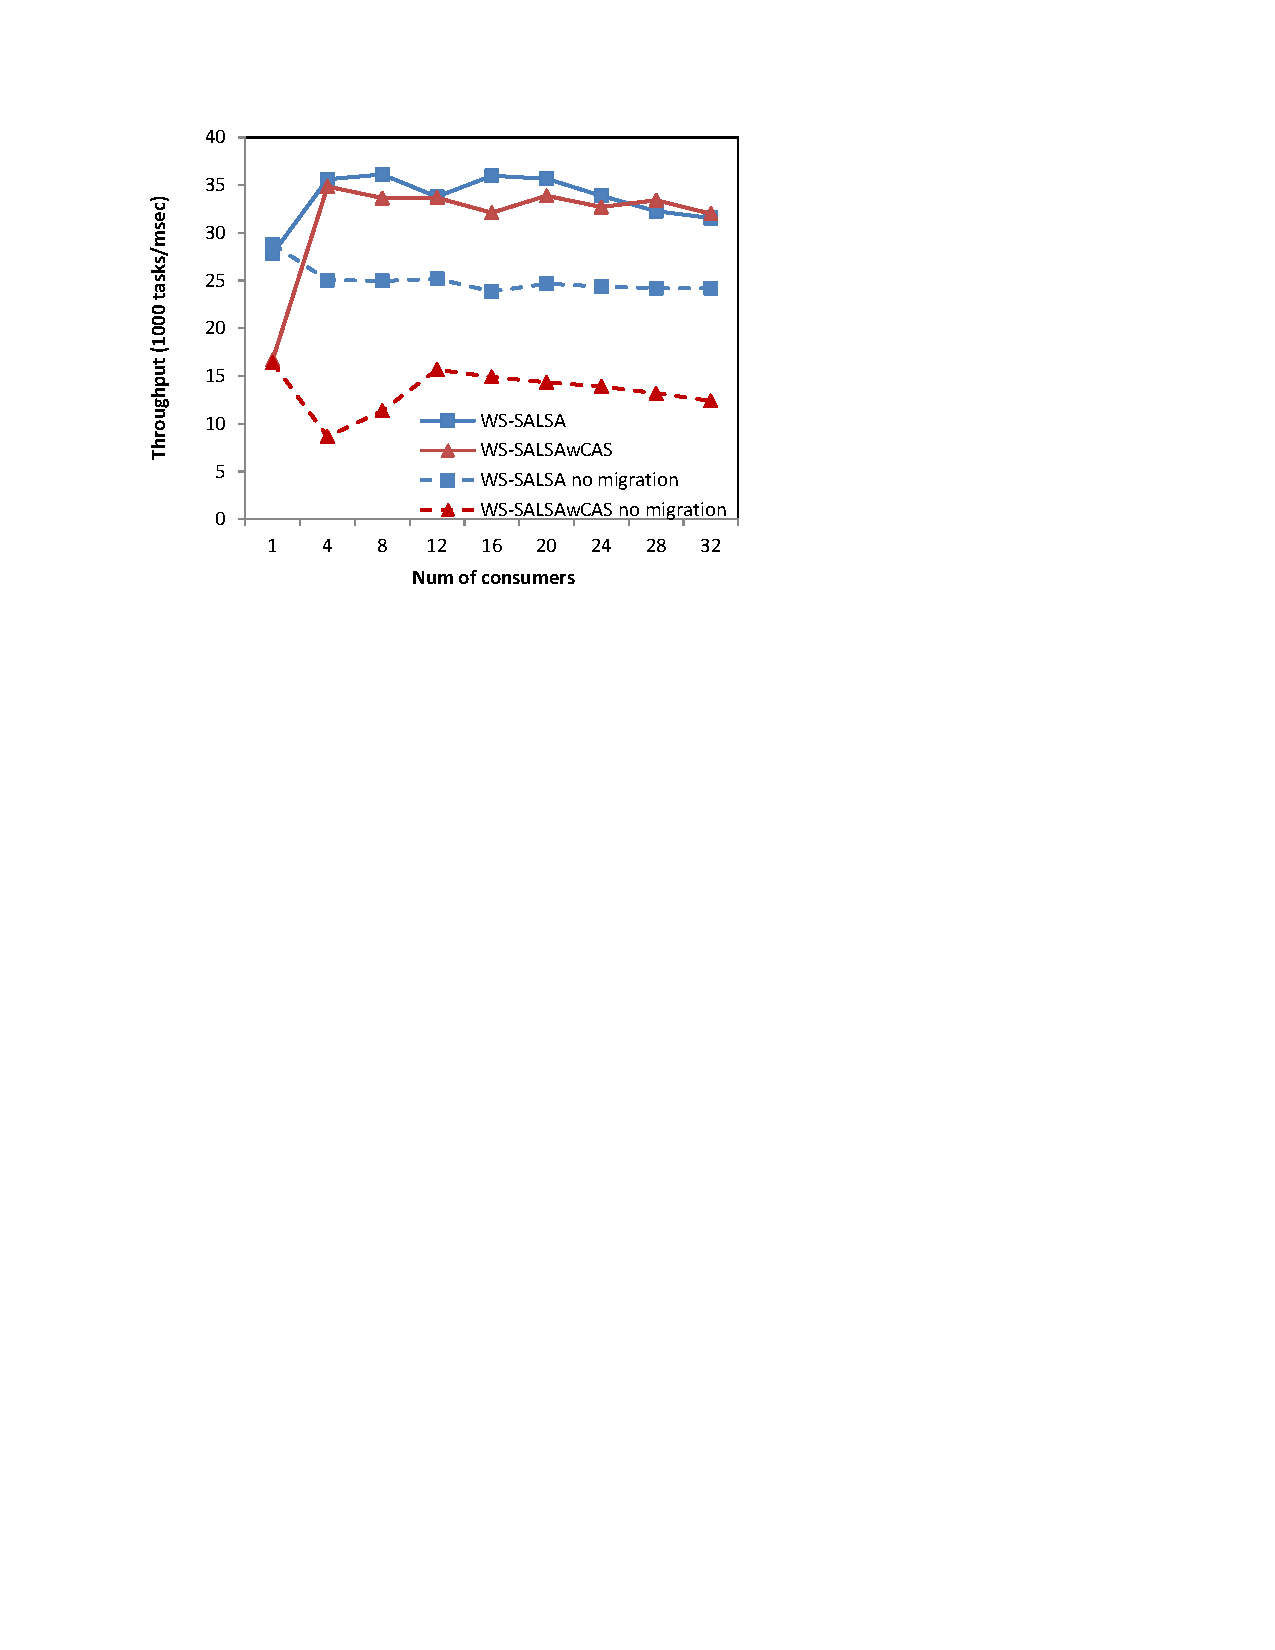
\includegraphics[width=0.40\textwidth]{figures/1-n-salsa}
    \label{fig:1-n-salsa-perf}
  }
  \subfigure [\scriptsize{CAS operations per task retrieval (1/N workload).}] {
    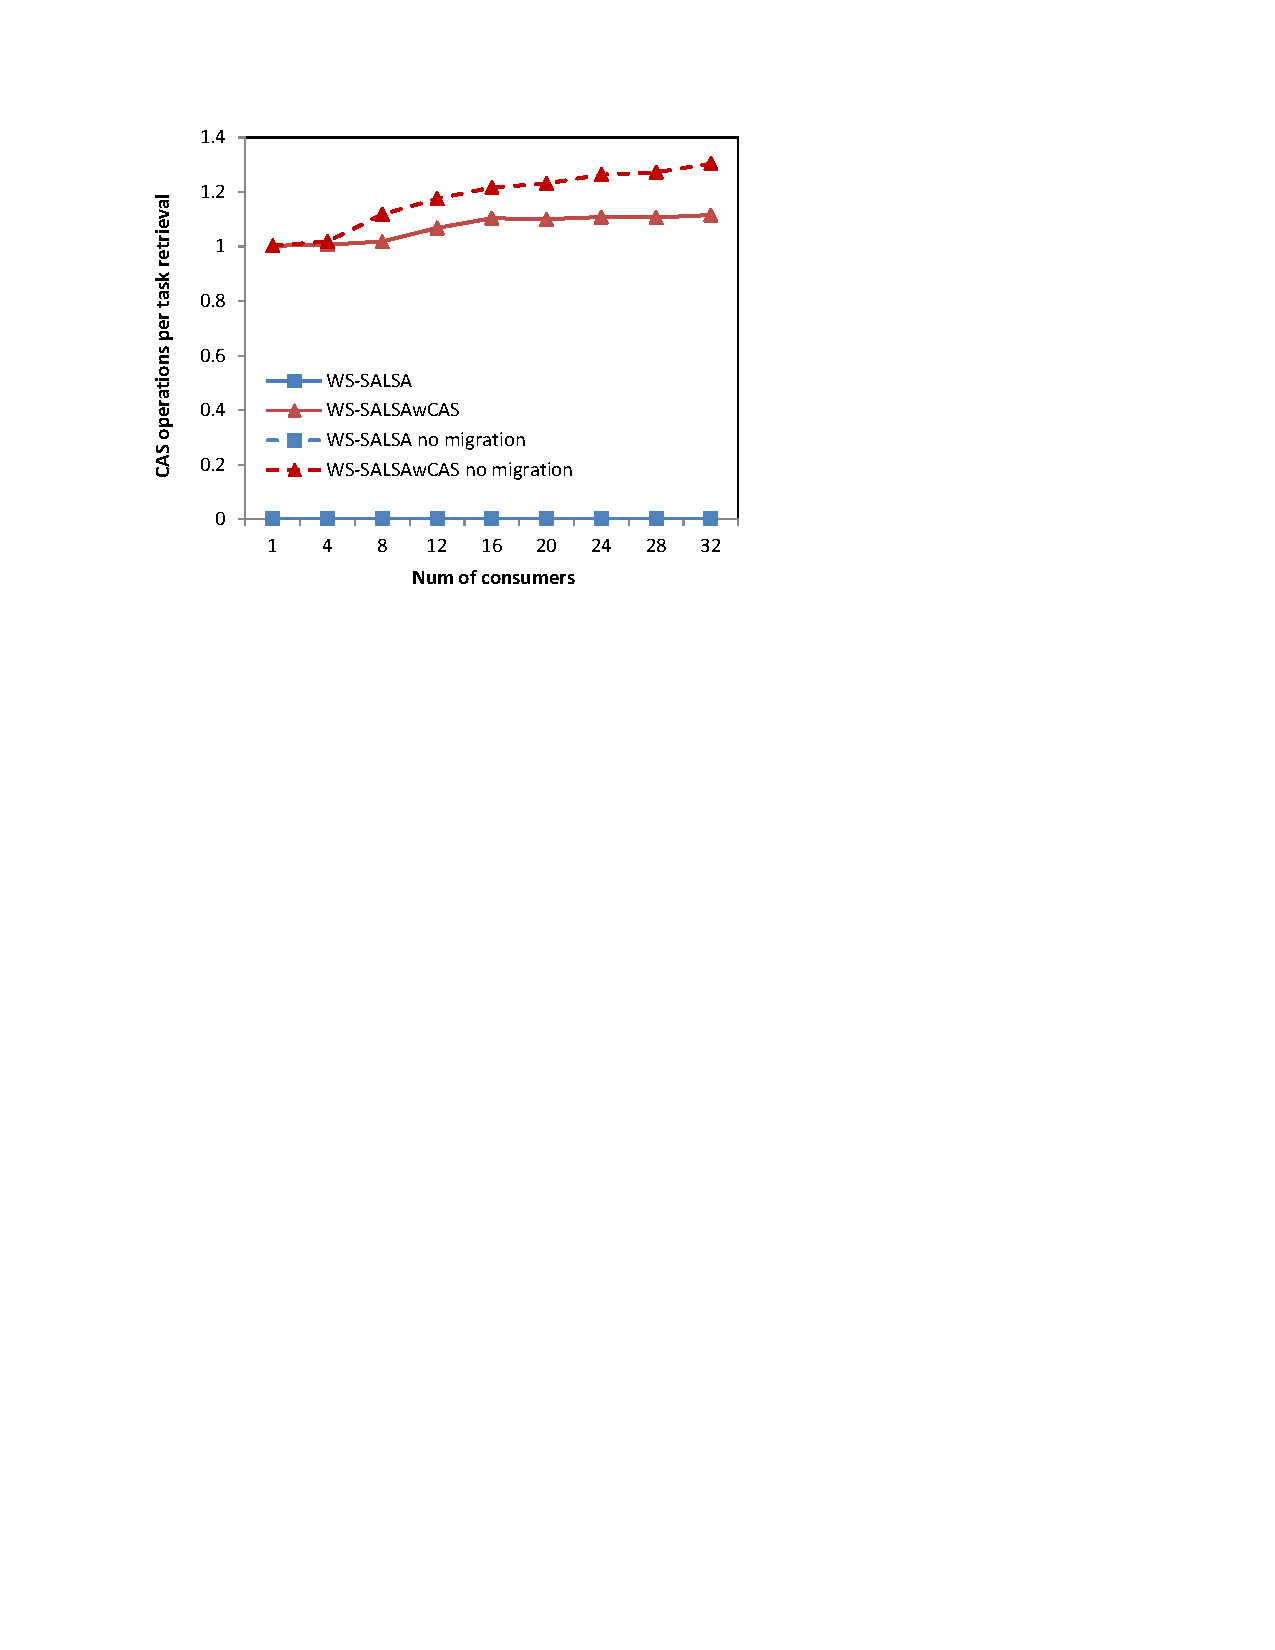
\includegraphics[width=0.40\textwidth]{figures/1-n-salsa-cas}
    \label{fig:1-n-salsa-cas}
  }
	\caption{\footnotesize{Single producer -- multiple consumers behavior. }}
	\label{fig:1-n-salsa}
\end{figure}

\begin{figure}[htb]
	\centering
	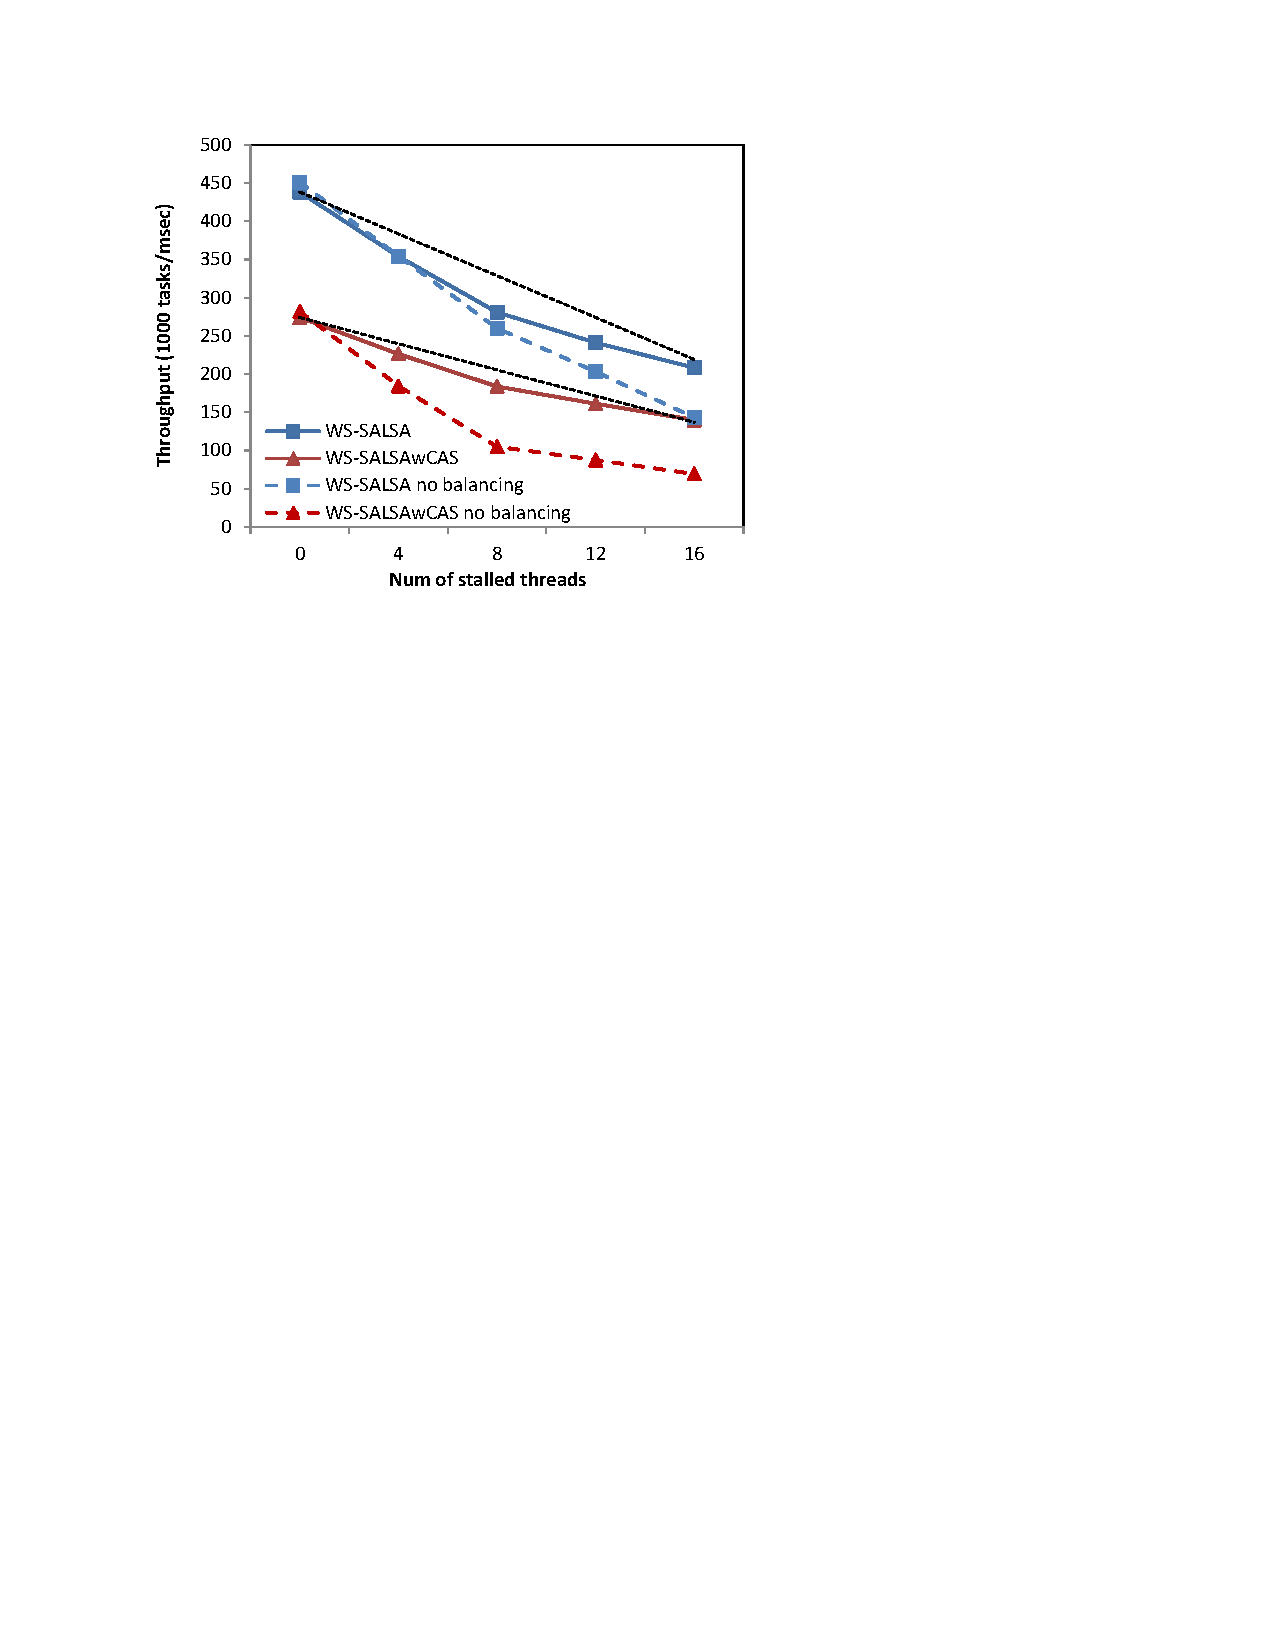
\includegraphics[width=0.40\textwidth]{figures/stalled-threads}
  \caption{\footnotesize{System throughput for different number of stalled threads (N/N workload). }}
	\label{fig:stalled-threads}
\end{figure}

\begin{figure}[htb]
	\centering
	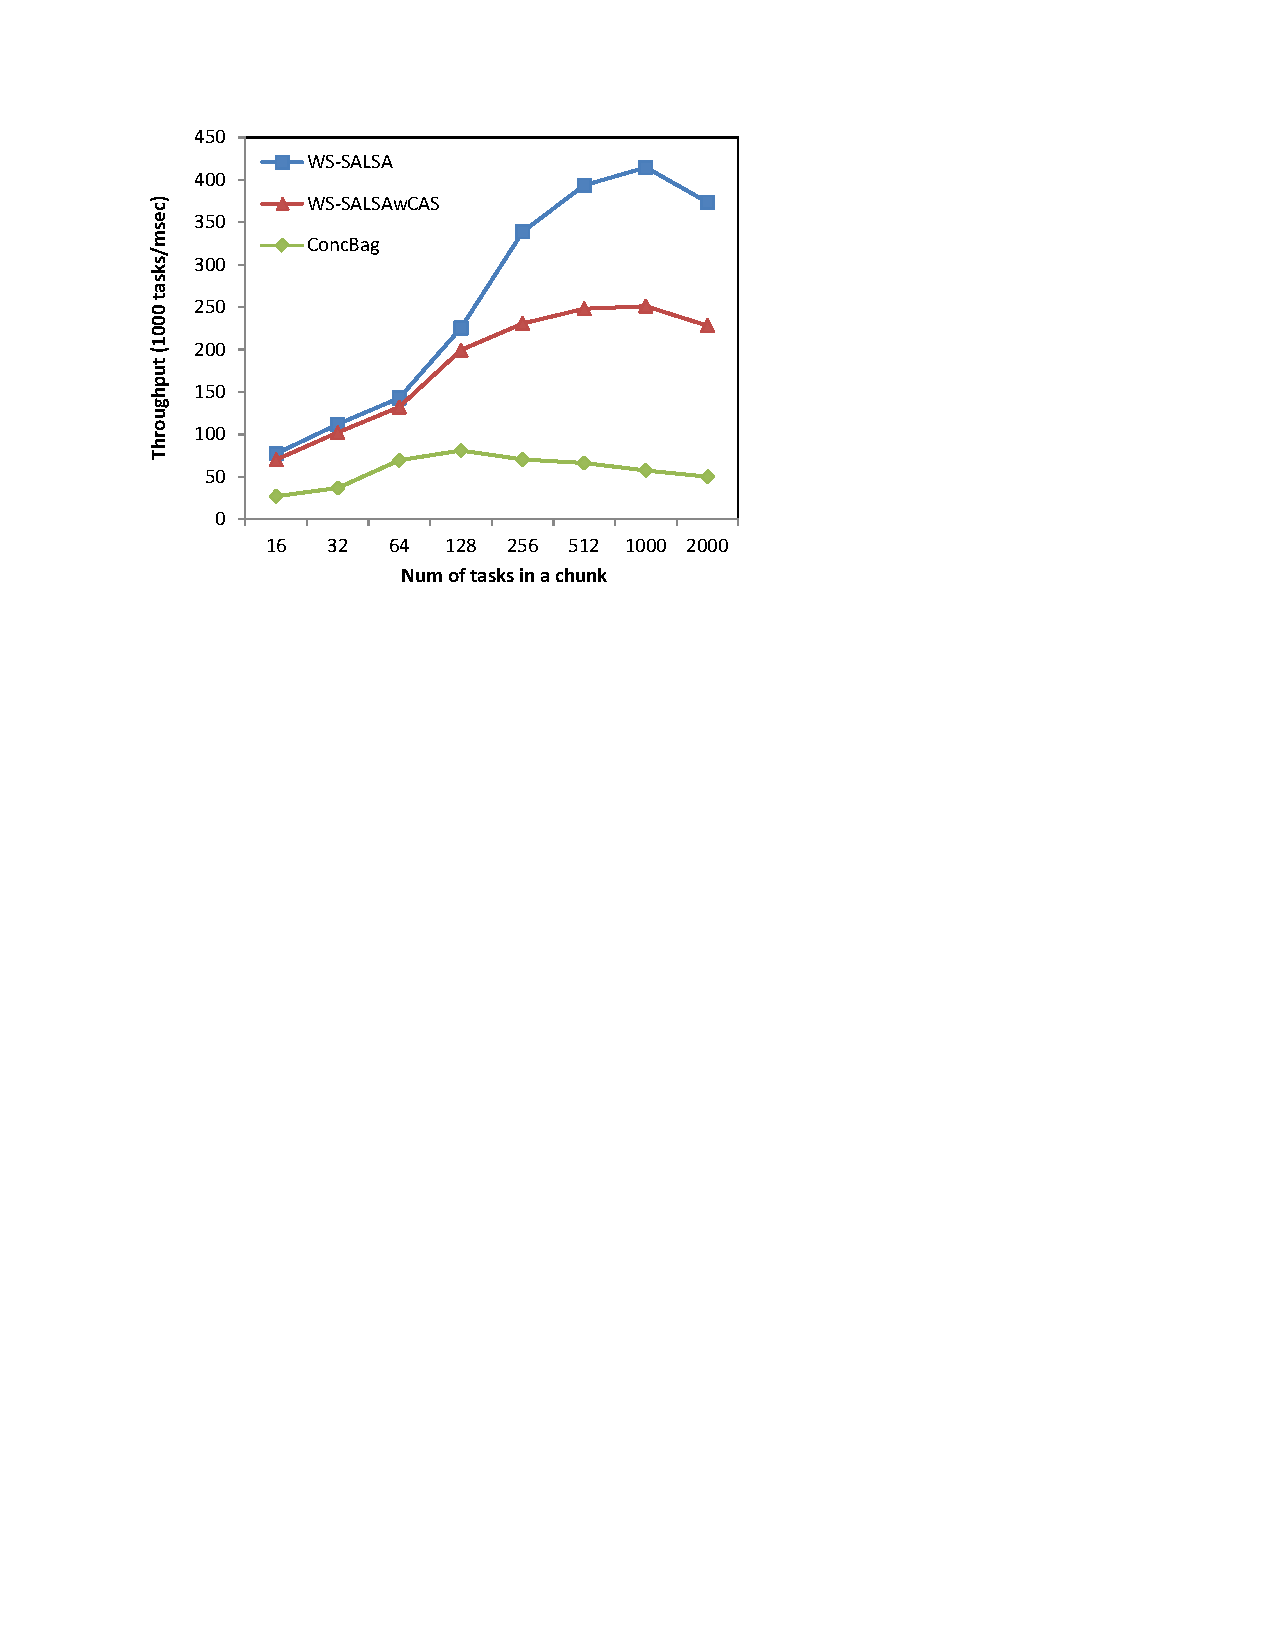
\includegraphics[width=0.40\textwidth]{figures/chunk-size}
  \caption{\footnotesize{System throughput as a function of chunk size. }}
	\label{fig:chunk-size}
\end{figure}